\documentclass[a4paper,10pt]{article}
\usepackage[utf8]{inputenc}

% ----  Useful packages % ---- 
\usepackage{amsmath}
\usepackage{graphicx}
\usepackage{amsfonts}
\usepackage{amsthm}
\usepackage{amssymb}
\usepackage{makecell}
\usepackage{array}
\usepackage{booktabs}
\usepackage{multirow}
% ----  Useful packages % ---- 

\usepackage{wrapfig}
\usepackage{caption}
\usepackage{subcaption}
\usepackage{hyperref}
\hypersetup{
    colorlinks,
    citecolor=black,
    filecolor=black,
    linkcolor=black,
    urlcolor=black
}

\graphicspath{ {./images/} }

% ---- Set page size and margins replace ------
\usepackage[letterpaper,top=2cm,bottom=2cm,left=3cm,right=3cm,marginparwidth=1.75cm]{geometry}
% ---- Set page size and margins replace ------

% ------- NOTA ------
\theoremstyle{remark}
\newtheorem{note}{Note}[subsubsection]
% ------- NOTA ------

% ------- OSSERVAZIONE ------
\theoremstyle{definition}
\newtheorem{observation}{Observation}[subsection]
% ------- OSSERVAZIONE ------

% ------- DEFINIZIONE ------
\theoremstyle{plain}
\newtheorem{definition}{Definition}[subsection]
% ------- DEFINIZIONE ------

% ------- ESEMPIO ------
\theoremstyle{definition}
\newtheorem{example}{Esempio}[subsection]
% ------- ESEMPIO ------

% ------- DIMOSTRAZIONE ------
\theoremstyle{definition}
\newtheorem{question}{Question}[subsection]
% ------- DIMOSTRAZIONE ------

% ------- TEOREMA ------
\theoremstyle{definition}
\newtheorem{theorem}{Teorema}[subsection]
% ------- TEOREMA ------

% ------- COROLLARIO ------
\theoremstyle{plain}
\newtheorem{corollaries}{Corollario}[theorem]
% ------- COROLLARIO ------

% ------- PROPOSIZIONE ------
\theoremstyle{plain}
\newtheorem{proposition}{Proposizione}[subsection]
% ------- PROPOSIZIONE ------

% ---- Footer and header ---- 
\usepackage{fancyhdr}
\pagestyle{fancy}
\fancyhf{}
\fancyhead[LE,RO]{A.A 2022-2023}
\fancyhead[RE,LO]{Systems Software}
\fancyfoot[RE,LO]{\rightmark}
\fancyfoot[LE,RO]{\thepage}

\renewcommand{\headrulewidth}{.5pt}
\renewcommand{\footrulewidth}{.5pt}
% ---- Footer and header ---- 

% ----  Language setting ---- 
\usepackage[italian, english]{babel}
% ----  Language setting ---- 

\usepackage{listings}
\usepackage{color}

\definecolor{dkgreen}{rgb}{0,0.6,0}
\definecolor{gray}{rgb}{0.5,0.5,0.5}
\definecolor{mauve}{rgb}{0.58,0,0.82}

\lstset{frame=tb,
  language=C,
  aboveskip=3mm,
  belowskip=3mm,
  showstringspaces=false,
  columns=flexible,
  basicstyle={\small\ttfamily},
  numbers=none,
  numberstyle=\tiny\color{gray},
  keywordstyle=\color{blue},
  commentstyle=\color{dkgreen},
  stringstyle=\color{mauve},
  breaklines=true,
  breakatwhitespace=true,
  tabsize=3
}

\title{\textbf{Telematics}}
\author{Autor: Ghirardini Filippo}
\date{Winter Semester 2024-2025}

\begin{document}
\begin{titlepage} %crea l'enviroment
	\begin{figure}[t] %inserisce le figure
		\centering
\includegraphics[width=0.98\textwidth]{marchio_unipi_pant541.png}
	\end{figure}
	\vspace{20mm}
	
	\begin{Large}
		\begin{center}
			\textbf{Dipartimento di Informatica\\ Corso di Laurea Triennale in Informatica\\}
			\vspace{20mm}
			{\LARGE{Corso a Libera Scelta - 6 CFU}}\\
			\vspace{10mm}
			{\huge{\bf Computer Graphics}}\\
		\end{center}
	\end{Large}
	
	
	\vspace{36mm}
	%minipage divide la pagina in due sezioni settabili
	\begin{minipage}[t]{0.47\textwidth}
		{\large{\bf Professore:}\\ \large{Prof. }}
	\end{minipage}
	\hfill
	\begin{minipage}[t]{0.47\textwidth}\raggedleft
		{\large{\bf Autore:}\\ \large{Filippo Ghirardini}}
	\end{minipage}
	
	\vspace{25mm}
	
	\hrulefill
	
	\vspace{5mm}
	
	\centering{\large{\bf Anno Accademico 2023/2024 }}
	
\end{titlepage}

\tableofcontents
\newpage
\maketitle
\begin{center}
    \vspace{-20pt}
    \rule{11cm}{.1pt} 
\end{center}
\newpage
\section{Basics}
\subsection{Network composition}
A network consists of three elements:
\begin{itemize}
	\item \textbf{End systems}: can vary in size and usage
	\item \textbf{Intermediate systems}: these (e.g. routers) are the components that allow the network to work.
	\item \textbf{Links}: they connect the end systems and can be \textit{optical}, \textit{copper} or \textit{wireless}. Even if wireless is becoming more and more important, cables are still fundamental (undersea cables, underground cables).
\end{itemize}

\begin{question}[Why fiber optic?]
	Because this medium has not reached it's maximum and still has a huge potential of \textbf{bandwidth}. Also, while copper cable start acting as an \textbf{antenna} (and a receiver), disturbing near copper cable, fiber optic doesn't have this problem. Furthermore, copper cables need amplifiers which increase \textbf{latency}.
\end{question}

\begin{question}[Why copper?]
	It's \textbf{cheaper} and \textbf{easier} to handle.
\end{question}

\begin{question}[Why cables over wireless?]
	Because of \textbf{stability} and \textbf{latency}. Usually the problem is tampered by buffers but obviously it doesn't work with interactive applications.
\end{question}

\begin{question}[What are threats to cable?]
	
\end{question}

\subsection{Communication principles}
There are two basics principles:
\begin{itemize}
	\item \textbf{Synchronous}: joint action of sender and receiver. Requires \textbf{waiting} until all parties are ready (e.g. phone calls)
	\item \textbf{Asynchronous}: sender and receiver operate decoupled (e.g. SMS, email). Requires \textbf{buffering}.
\end{itemize}

\begin{note}
	There is also \textbf{isochronous}, which means the messages are sent every predetermined amount of time.
\end{note}

\subsubsection{Direction}
Communication channels may allow traffic flow in different directions:
\begin{itemize}
	\item \textbf{Simple duplex}: one direction
	\item \textbf{Half-duplex}: both directions in different moments
	\item \textbf{Full-duplex}: both directions at the same time
\end{itemize}
\subsubsection{Distribution}
The communication distribution can happen in different ways:
\begin{itemize}
	\item \textbf{Unicast}: one to one
	\item \textbf{Broadcast}: one to all
	\item \textbf{Multicast}: one to a subset
	\item \textbf{Anycast}: one to the nearest, e.g. when requesting to a redundant database you don't care which one responds
	\item \textbf{Concast}: many to one, e.g. we collect sensor data and send it to one
	\item \textbf{Geocast}: one to a certain region
\end{itemize}
\begin{note}
	Even if multicast would be easier and cheaper, companies usually go for unicast because they want to know who the clients are.
\end{note}

\begin{note}
	Broadcast guarantees anonymity while multicast does not.
\end{note}

\subsubsection{Topologies}
The main topologies are:
\begin{itemize}
	\item \textbf{Full mesh}: too expensive
	\item \textbf{Chain}: in cars and trains
	\item \textbf{Star}: ideal for switches
	\item \textbf{Partial mesh}: the best compromise
	\item \textbf{Tree}: not ideal for big networks since if you cut a side, you lose contact
\end{itemize}

\subsection{Sharing}
\subsubsection{Cons}
Sharing may create a lot of problems, like \textbf{bottlenecks}: links and intermediate nodes are shared between end systems. One solution may be to \textit{reroute} or to start \textit{dropping packets} (e.g. when streaming the resolution lowers down).
\subsubsection{Pros}
At the same time, sharing means more efficient (less expensive) mechanism to \textbf{exchange data} between different components of distributed systems and \textbf{minimize blocking} due to multiplexing.

\subsubsection{How?}
There are two possible ways of sharing:
\begin{itemize}
	\item \textbf{Reservation}: you reserve in advance the resource so that it is guaranteed, e.g. remote surgery. When the peak demand and the flow duration varies, there are two options:
	\begin{enumerate}
		\item \textit{First Come First Served}
		\item Everyone gets $10Mbps$
	\end{enumerate}
	It is implemented with \textbf{circuit-switching}: establishes dynamically a dedicated communication channel. It has predictable performance and a simple and fast switching but it's inefficient for bursty traffic, complex to setup and not easily adaptive to failures.
	
	\item \textbf{On-demand}: when there is a resource available you take it (variable \textit{delay}, \textbf{jitter}), e.g. email. It is implemented with \textbf{packet-switching}: splitting the resource in packets and multiplex them. Much more flexible but requires buffers, packets overhead and has unpredictable performances.
\end{itemize}

\begin{observation}
	It all depends on the application. Each flow has a \textbf{peak rate} and an \textbf{average rate}.To decide if \textit{reservation} works well for a specific case, we must look at the ratio $\frac{P}{A}$. If it's small then it works well, otherwise it's wasting resources.
\end{observation}
\newpage
\section{DNS}
\subsection{Introduction}
Names provide a level of abstraction from the IP address: for humans it's easier to remember. It also provides \textbf{load balancing} and easy \textbf{aliasing}.\\
The decision for DNS adding is handled by two organizations:
\begin{itemize}
	\item \textbf{IETF}: how entries are entered and read from the phone book
	\item \textbf{ICANN}: how to decide \textit{what} names should be entered in the phone book
\end{itemize}
To use naming you need two things:
\begin{itemize}
	\item \textbf{Unique} names
	\item \textbf{Resolution} of names to locator (IP address) or other services
\end{itemize}

\subsubsection{Scaling}
To allow scaling, DNS uses \textbf{delegation} and \textbf{caching}. In particular for delegation, DNS adopts three intertwined \textbf{hierarchies}:
\begin{itemize}
	\item \textbf{Name space}: hierarchy of names
	\item \textbf{Management}: hierarchy of authorities over names. Who owns which name part.
	\item \textbf{Infrastructure}: hierarchy of DNS server. Where is the mapping stored.
\end{itemize}

\subsection{Namespace}
DNS namespace is implemented as a tree structure: each node has a \textbf{label} which identifies it relatively to its parent node. Each node is \textbf{root} of a sub-tree (if it's not a leaf). In particular direct children of the root are called \textbf{Top Level Domains}. Each subtree represents a \textbf{domain} and each domain can be divided in \textbf{sub-domains}.
\begin{center}
	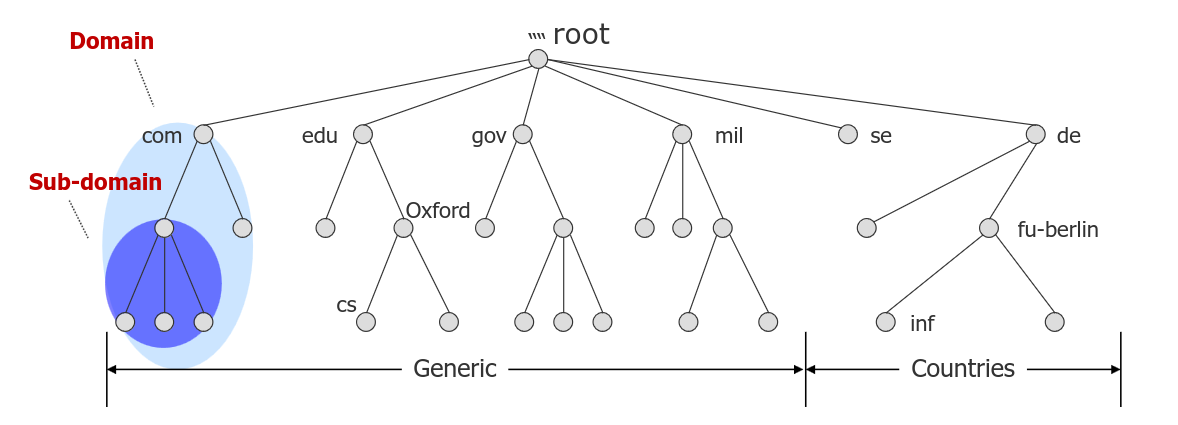
\includegraphics[scale=0.3]{dns_hier.png}
\end{center}
There is a limited number of TLDs: originally it was $7$ plus one for each country. Now there are many more, even in non Latin alphabets.
\subsubsection{Leafs}
The name of a domain consists of a sequence of labels beginning with the root of the domain and going up to the root of the whole tree. Each label is separated by ".".\\
In the leaf nodes the IP addresses are associated with the names.\\
Furthermore, there could be \textbf{Domain Name Aliases}: pointers of one domain to another (Canonical Domain Name).

\subsubsection{DNS Database}
There are a few rules for the database:
\begin{itemize}
	\item The \textbf{depth} of the tree is limited to $127$
	\item Each label can have up to $63$ characters
	\item The whole domain name has a maximum of $255$ characters (even if the average is $10$)
	\item A label of length $0$ is reserved for the root
\end{itemize}
The full address to a host is the \textbf{Fully Qualified Domain Name}, which includes the leaf, each node and the root. The \textbf{Relative Domain Name} instead, is an incomplete domain name.

\subsection{Management}
The management of domain names also follows a hierarchy structure: \textbf{ICANN} manages the root domain and delegates someone (\textbf{DENIC} for Germany) to handle the \textit{de} domain. They then delegate FUB to handle the \textit{fu} domain. And so on.\\
This solution ensures that the names are unique.

\subsection{Name servers and zones}
\subsubsection{Domains}
Domains are administrative concepts managed by single organizations. The name of the domain corresponds to the name of the root node. They can delegate the responsibility for subdomains to other organizations but maintains the pointer to them to be able to forward requests.
\subsubsection{Name servers and zones}
On the other hand, name servers and zones are technical concepts. The name server is a process that maintains a database for a domain space. The part of the name space known to the server is called a \textbf{zone} and it's stored in a \textit{zone file}. The name server may have multiple zones and has authority over them.
\paragraph{Primary Master} It's a name server that must exist. Reads the data from a local file and has a database describing subdomains and computer in a selected zone.
\paragraph{Secondary Master} It's optional and is a replication of the master for reliability reasons. It receives the data from another server which is authoritative.

\subsection{Resolution}
There are two types of Name Resolution:
\begin{itemize}
	\item \textbf{Recursive}: the name server replies either with the answer or with an error and it's responsible to contact the other nodes
	\item \textbf{Iterative}: a name server replies with the address of another one, it's the host duty to contact additional name servers for the answer
\end{itemize} 

\begin{question}[Why do root servers not support recursive solution?]
	Using the recursive option implies that every intermediate needs to wait for all the others, depleting its resources.
\end{question}

\begin{question}[How does this all contribute to scalability?]
	We do not have \textbf{strong consistency} and 
\end{question}

\subsubsection{Reverse lookup}
While mapping a name to a \textit{global} IP address is simple, doing the other way round it's really difficult because we need to do a complete search of the tree. \\
Because of this, there is a special area in the database called \textbf{in-addr.arpa} that contains $256$ sub domains, each one having $256$ and so on.
\begin{center}
	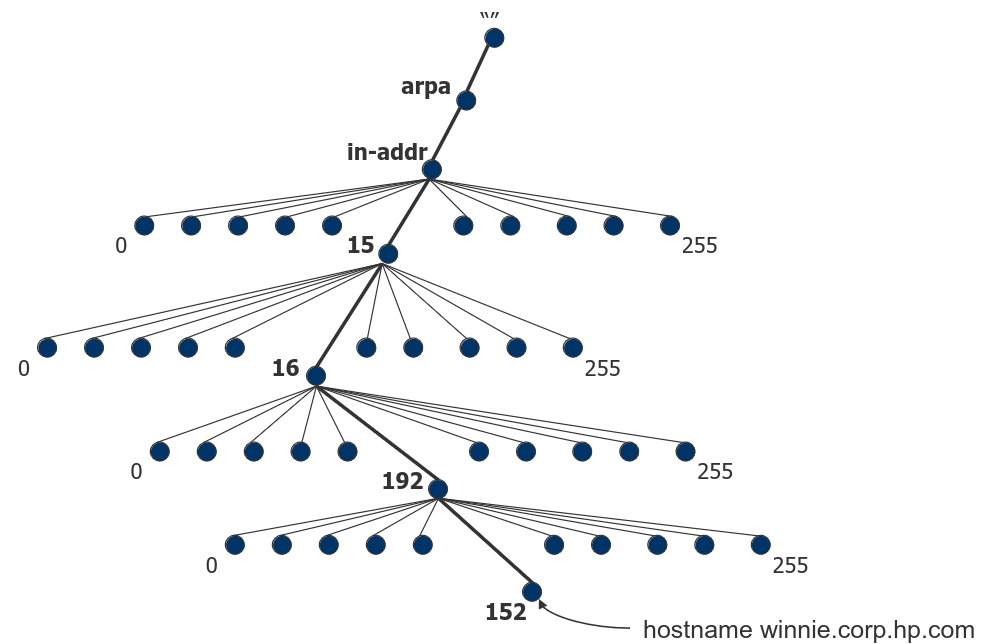
\includegraphics[scale=0.3]{reverselookup.png}
\end{center}
\begin{note}
	This is useful against \textbf{spoofing}: as an example if you get an email and you want to check if the sender is who claims to be, you can do a reverse lookup on the IP of the email server.
\end{note}

\begin{question}[Why does reverse lookup not always work?]
	Because the entries are not always present in the database.
\end{question}

\subsection{Database entries}
A \textbf{resource record} is the entry in the database to get the address or other information of a name. It's composed of a tuple:
\begin{lstlisting}[language=Python]
	(name, TTL, class, type, value)
\end{lstlisting}
\paragraph{TTL} It's the Time To Live: after a certain amounts of seconds the record will be deleted from the cache and updated. With a shorter TTL you have a very updated cache while longer TTL means outdated caches but less requests for the server.
\paragraph{Type} Indicates the type of data to be returned. \textbf{A} is the actual IPv4 address corresponding to the name (\textbf{AAAA} for IPv6). 
\paragraph{Class} Nowadays it's only \textbf{IN} but there were in the past other options for different networks with independent DNS zones.

\begin{observation}[Load balancing]
	DNS is very useful for load balancing: depending on the region when you ask for a DNS entry the answer will be the closest one. It can also be used for \textbf{evil purposes} (censorship, marketing).
\end{observation}

\subsubsection{Name Server}
For each name server of a zone a \textbf{Name Server} record is created in the cache. E.g. when you want to visit \textit{arnold.movie.edu} you may have in cache a NS entry for \textit{movie.edu}.

\subsubsection{CNAME}
A \textbf{CN} record is an optional entry in the database that illustrates aliases on its canonical names. 

\subsubsection{Pointer}
The \textbf{PTR} record provides information for the mapping of an address to names. If you do not have any entry for an IP address you then have to do a reverse lookup. Addresses should refer only to one name.

\subsubsection{Mail Exchanger}
The \textbf{MX} record serves for the controlling of the email routing. It specifies an email server responsible for a domain name with the option to indicate a preference if multiple servers are present (the smallest value is preferred).

\subsection{Protocol}
The resolver software triggers the resolution process and tries first for the cache. Then it sends the request to the local DNS server which is either static (resolv.conf) or dynamic (DHCP). \\
The protocol consists of a single packet used for inquiries and responses:
\begin{center}
	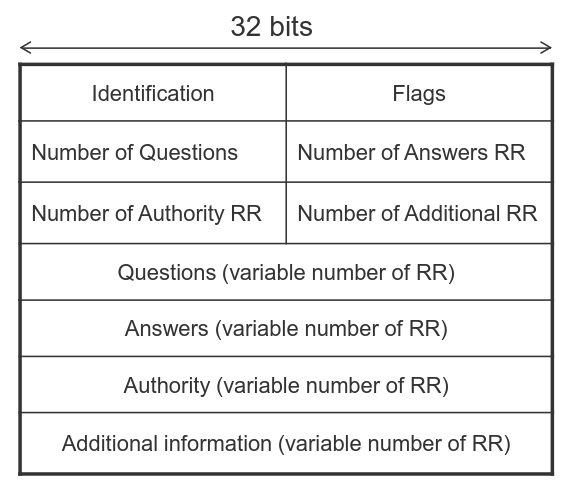
\includegraphics[scale=0.3]{dns.png}
\end{center}
\paragraph{Identification} $16bits$ for the mapping of an inquiry to a response.
\paragraph{Flags} $16bits$ of various flags that indicate if the packet is a request or a response, if it's \textbf{authoritative} or not, if it's \textit{iterative} or \textit{recursive}.
\paragraph{Numbers} These fields indicate the contained number of inquiries responses data records.
\paragraph{Questions} Contains the names to be resolved.
\paragraph{Answers} Resource records to the previous inquiry.
\paragraph{Authority} Contains the ID of the passed responsible NS.
\paragraph{Additional information} If the name searched is only an alias, the belonging resource record for the correct name is placed here.

The packet is sent through UDP on port $53$ and the \textbf{reliability} is only implemented via repeating the requests. Also it is not protected.

\subsection{Scalability}
The scalability is achieved mainly with local caching of recent results. The cache can be in the network and also in the local client.\\
One of the main problem is how long should you keep the entries? You need to achieve both \textbf{consistency} and not doing too many requests. You also need to detect and flush the \textbf{stale entries}. You have to avoid \textbf{cache poisoning}: when a malicious person changes the value in the cache to redirect you to an evil software.
\subsection{Extension}
\subsubsection{Dynamic DNS}
The problem comes up when, as an example, you restart the router and your public IP address is changed (or maybe the ISP changes it every 24 hours). The DDNS allows you to tell the changed IP address.
\subsubsection{Characters}
The original DNS supports only ASCII, so there is an extension for UTF characters.
\subsubsection{DNSSEC}
The \textbf{security} is important because DNS is the most crucial indirection to access the data. Controlling DNS response implies controlling the discovery of the communication endpoints. It may be use in an evil way for political and economical reasons.
\newpage
\section{Email}
\subsection{Introduction}
Email is an example of an application that works on the different layers. It's \textbf{asynchronous}, \textbf{decentralized} (to improve \textit{scaling}), \textbf{client-server} and based on simple ASCII text.
\subsubsection{Motivation}
Email was the first \textit{killer application}. It started in the 1980's with a simple terminal interface, evolving in the 1990's with the \textit{web-mail} and then \textit{mobile email}. Today social network are trying to swallow the email concept.
\subsection{Architecture}
There are two actors involved:
\begin{itemize}
	\item \textbf{User Agent}, with email clients. Runs on the computer of the user and is intermittently on. E.g. Thunderbird or Outlook
	\item \textbf{Message Transfer Agent}: the email servers. They run on a remote machine and stores and forwards on behalf of the User Agents. It's always on
\end{itemize}

\begin{center}
	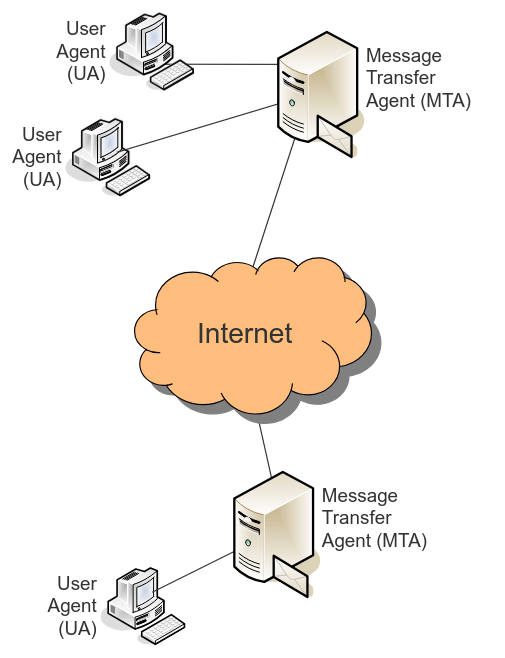
\includegraphics[scale=0.3]{email.png}
\end{center}

\subsection{Message}
Message are viewed as having an \textbf{envelope}, the fundamental part for the delivery, and a \textbf{content}. The latter contains a \textbf{header} with a certain coding and a \textbf{body} consisting of simple characters.

\subsubsection{Envelope}
The envelope is created by the \textbf{MTA} or the \textbf{MSA} and includes all the information for transporting the message. Some information are redundant with the header (like the sending and receiving address) but there are some differences, like when you send a Blind Carbon Copy message.

\begin{note}
	You can't know if the sender is correct. This can be used for evil purposes. The only way to avoid that is by encrypting or signing the email.
\end{note}

\newpage
\subsubsection{Content}
\paragraph{Header} It contains characters with the following syntax:
\begin{lstlisting}
	<key>:<value>
\end{lstlisting}
\paragraph{Body} It's the content of the email. It's separated from the header by a blank line.

Since originally the content could only contain $7bit$ ASCII, \textbf{Multipurpose Internet Mail Extensions} was invented to extend the classical format. It adds additional headers, content types and sub-types:
\begin{itemize}
	\item \textbf{MIME-version}
	\item \textbf{content-description}: string that describes the content of the message
	\item \textbf{content-id}: identifier for the content
	\item \textbf{content-transfer-encoding}: selected coding for the content (BASE64, ASCII)
	\item \textbf{content-type}: specifies the type of the body in the format \textit{type/subtype}, e.g. text, image, audio, video, etc..
\end{itemize}

\subsection{Protocols}
\subsubsection{SMTP}
Simple Mail Transport Protocol delivers the mail to the final inbox. It can't ensure that the message arrives to the final user because it expects the receiver to be always online.\\
It uses \textbf{reliable data transfer} based on TCP on port $25$ and it's \textit{best effort}. It provides \textbf{little security}: no encryption, optional authentication on port $587$ to reach MSA but nothing between MTAs.\\
The protocol follows these steps:
\begin{enumerate}
	\item \textbf{Write} an email, the client formats it and sends it to it's own mail server
	\item The mail server sets up a connection with the receiver's server and \textbf{sends} a copy of the email
	\item The \textbf{receiver}'s server creates the header of the email and places the message in the inbox
\end{enumerate}

\paragraph{Graylisting} A first attempt to block spam. If a combination of IP address of the sender, their email and the receiver's one is seen for the first time, the message is discarded and an error is returned. From the second time on, the message goes through. This is based on the idea that scammers won't send the email twice.

\subsubsection{POP3}
This protocol pulls emails from the server over a connection on port $110$. It's text based and allows basic functionalities such as \textit{logging}, \textit{copying locally} and \textit{deleting} from the server.\\
It works in two phases:
\begin{enumerate}
	\item \textbf{Authorization} phase: \textit{user}name and \textit{pass}word for authentication, either successful or not
	\item \textbf{Transaction} phase: a \textit{list} of the messages and their sizes is provided, then via \textit{retr} its possible to retrieve a message using the number of the list and with \textit{dele} to delete an email.
\end{enumerate}

\begin{note}
	POP3 is heavily limited due to problems with multiple users handling and always-on connections.
\end{note}
\subsubsection{IMAP}
This protocol works on port $143$. In this case the emails remains on the server and may be cached by the client. All the actions are performed on the server. Ideal when you need to access it from different locations.

\subsubsection{HTTP}
The \textbf{webmail} allows the user to interact with emails via WEB. E.g. Gmail or Outlook.
\newpage
\section{HTTP}
HTTP is a protocol that allows the user to request a \textbf{resource} (e.g. HTML page) that is on a server. They may contain references to other resources, therefore creating a \textit{web}, called \textbf{World Wide Web}.
\subsection{History}
The first idea came in 1945 by Vannever Bush, with his \textbf{Memtex}, a desk containing different information categorized accordingly: \textbf{hypertex} context was born. Then in 1962 Doug Engelbart started to work on its actual implementation and by 1989 Tim Berners Lee connected that with TCP/IP and DNS protocols, effectively creating the WWW. \\
Today it gives access to \textbf{intelinked documents} distributed across several computers in the world, using the internet as exchange.

\subsection{Communication}
\subsubsection{HTTP/1}
The standard way of communicating is between a \textbf{client} (e.g. Firefox, Chrome) and a \textbf{web server} (e.g. Apache, Nginx).\\
The communication is handled by the HTTP protocol (usually on port $80$). It's a text based \textbf{request/response} protocol.\\
It was \textbf{stateless} until version 2. This means that the server maintains no information about previous requests and thus the specification of the context is needed every time.\\

\paragraph{Request} HTTP requests follow the \textbf{REST} API principle, allowing for performance, scalability, simplicity, modifiability, portability and reliability. The resources are retrieved via a \textbf{URL}

\begin{center}
	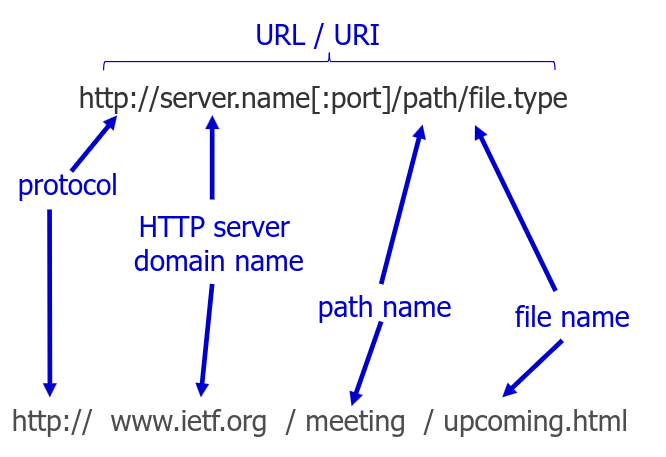
\includegraphics[scale=0.3]{url.png}
	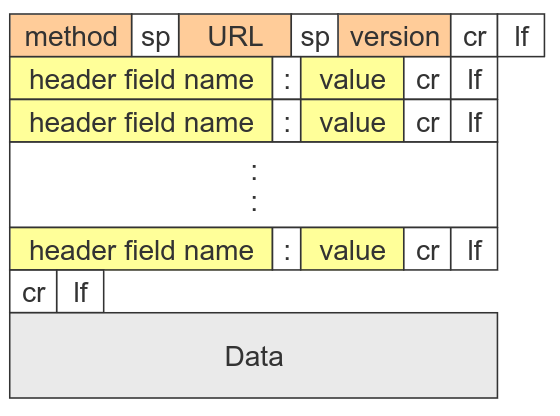
\includegraphics[scale=0.3]{httpreq.png}
\end{center}

\noindent The specified commands that can be used with a URL are:
\begin{itemize}
	\item \textbf{GET}: load a web page
	\item \textbf{HEAD}: load only the header of the web page, used for \textit{debugging}
	\item \textbf{PUT}: store a page on the web server
	\item \textbf{POST}: append something to the request passed to the web server
	\item \textbf{DELETE}: delete a web page
\end{itemize}

\newpage
\paragraph{Response}  The HTTP response contains the protocol used, the header lines and the \textbf{status code} , that can be:
\begin{itemize}
	\item \textbf{1xx}: only for information
	\item \textbf{2xx}: successful inquiry
	\item \textbf{3xx}: further activities are necessary
	\item \textbf{4xx}: client error (syntax)
	\item \textbf{5xx}: server error
\end{itemize}
\begin{center}
	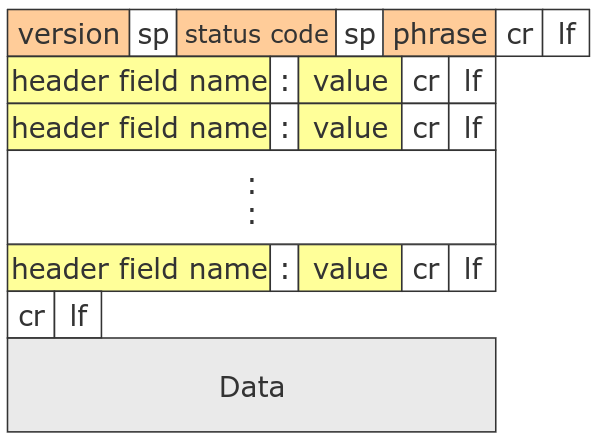
\includegraphics[scale=0.3]{httpresp.png}
\end{center}

\subsubsection{Web Sockets}
HTTP first problem is that the client needs to poll explicitly for content, causing a huge \textbf{overhead}. Thus Web Sockets were created: they allow a full duplex communication between the server and the client without the need of HTTP. It uses the same ports and it's set up using an HTTP request to "upgrade", which is then answered with a "switching protocol" response.

\subsubsection{WebRTC}
HTTP second problems is to enable communications between multiple browsers without creating a web server for each one of them. WebRTC implements a P2P communication that provides functions to establish media and data exchange, e.g. for videoconferencing.

\subsubsection{HTTP/2}
The second version of HTTP is \textbf{binary} instead of text based. It is fully \textbf{multiplexed}, associating requests and response and allowing a bi-directional stream. Therefore it can use only one connection while still granting \textbf{parallelism}. Furthermore it uses \textbf{header compression} to reduce overhead and allows server to push responses into client caches, reducing the number of requests to render web pages.
\begin{center}
	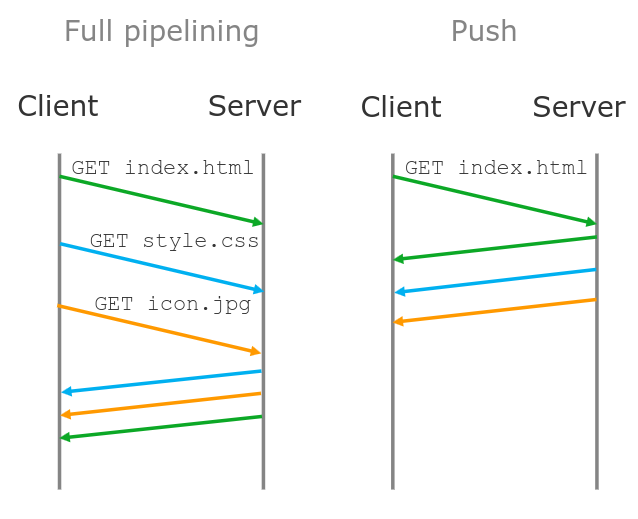
\includegraphics[scale=0.25]{http2.png}
\end{center}
\subsubsection{HTTP/3}
This version uses \textbf{QUIC} protocol over UDP instead of TCP and TLS for security, avoiding \textit{head of line} blocking.

\subsection{Cookies}
The main problem with HTTP is that it's \textbf{stateless}, this meaning that after every request/reply the web server forgets everything. While this is not a problem for simple browsing, it means that we cannot store user content to personalize the experience.\\
The solution is the \textbf{cookies}: tags stored in the web browser and set by the server so that they can be sent again to allow the latter to identify the client.\\
\subsubsection{Structure}
Cookies are stored as name-value pairs defined by the server. They can have optional parameters such as an \textbf{expiry date}.
\begin{center}
	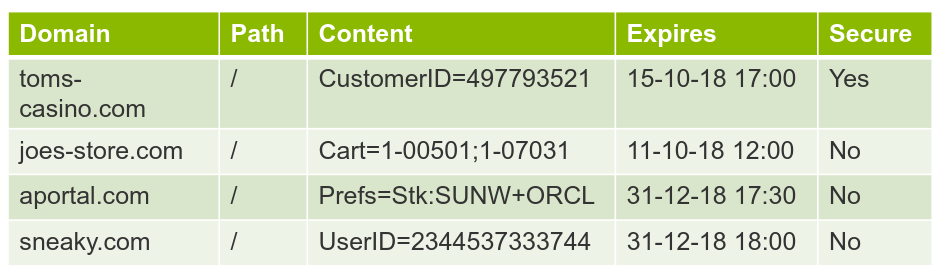
\includegraphics[scale=0.4]{cookies.png}
\end{center}

\subsubsection{Pros and cons}
They enable \textbf{authorization}, shopping carts, recommendations and \textbf{user session state} (e.g. for web mail). The biggest problem is about \textbf{privacy}: cookies are identified by \textbf{Etags}, an opaque identifier for a specific version of a resource, and can be used to track users.

\subsection{Proxy}
A \textbf{proxy} is an intermediate cache between multiple clients and a server. The main goal is to have a more \textbf{efficient} page loading, improving \textbf{scalability}. It temporarily stores the pages loaded by the browsers: if the client requests it and it hasn't changed yet, it's loaded from the proxy, otherwise a new request to the server is made and the cache is updated.\\
It can also enable support for protocols such as FTP or Telnet without the need for a new browser implementation.\\
It can also work as a \textbf{firewall}. 

\subsection{Scaling}
To handle huge loads (top 1000 websites) we use \textbf{3-tier} architecture, which separates the web server in \textbf{presentation servers}, \textbf{logic servers} and \textbf{database storage}. 
\begin{center}
	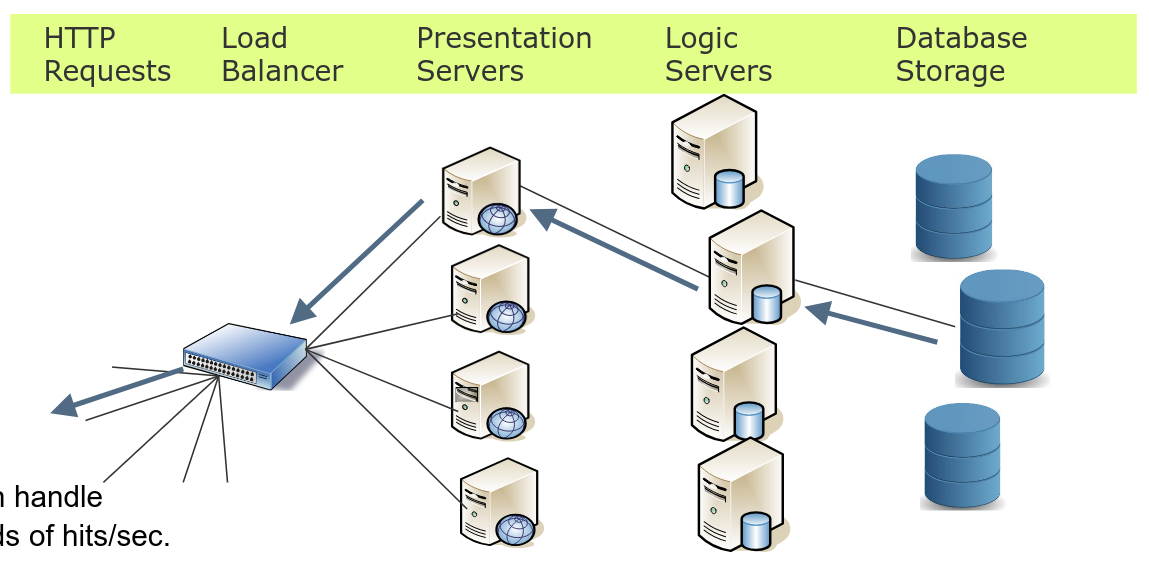
\includegraphics[scale=0.25]{3tier.png}
\end{center}
If, instead, we want to deal with medium and small web servers, we usually virtualize a lot of them on a single machine and we do the multiplexing with the server URL field in HTTP.

\subsection{DNS}
It's possible to use DNS over HTTP by sending a request (either \textit{GET} or \textit{POST}) to the DNS server. It improves privacy and security but the user looses control.
\end{document}
